% vim: set filetype=tex

\section{\color{fancy}Chapter 4: Table View}

\begin{figure}[h]
  \centering
  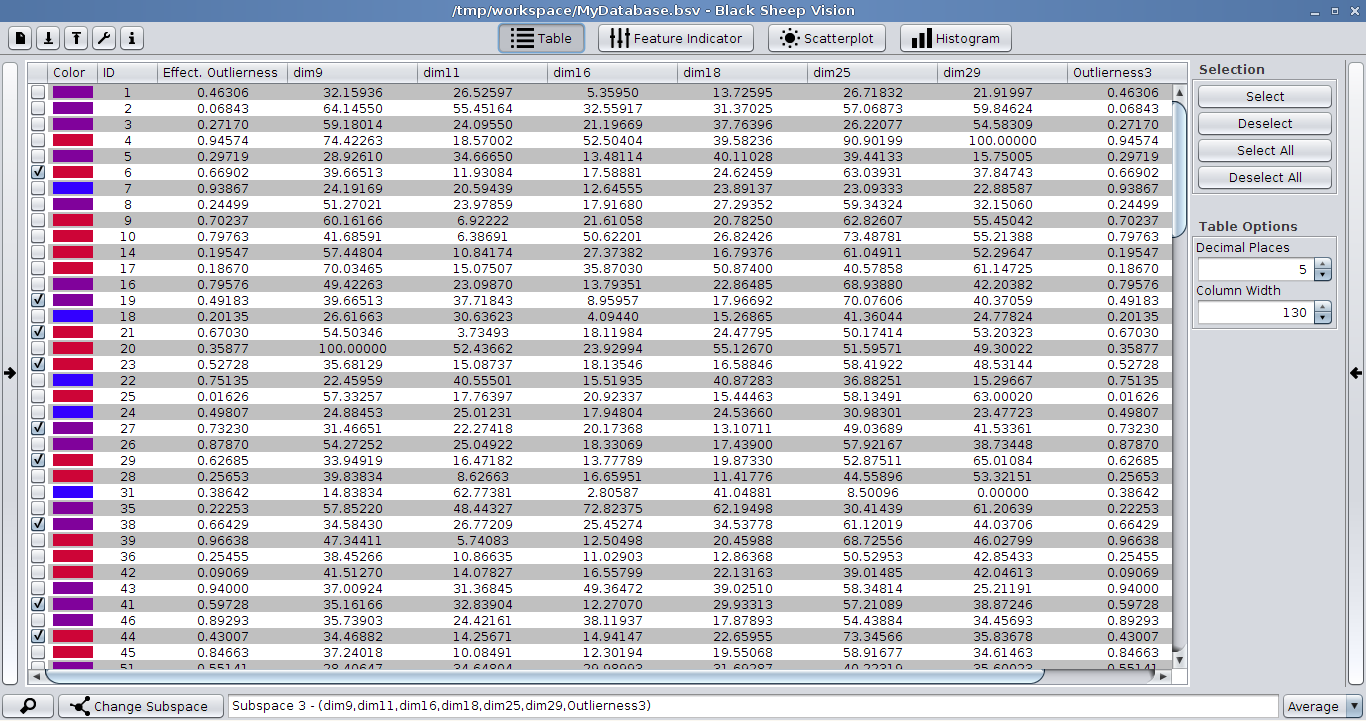
\includegraphics[width=16cm]{images/bsv/TableView.png}
  \caption{Table View}
  \label{fig:tableview}
\end{figure}

\subsection{Functionality}
\begin{tabular}{p{0.2\linewidth}p{0.7\linewidth}}
  \color{fancy}Feature & \color{fancy}Usage \\ \hline
  Display & The Table View gives you a simplistic dump of your data, combined with information about specific IDs and their group membership, easily recognizable by their color field. \\ \hline
  Control & On the right side you find various buttons, to control the table's behavior, for example the decimal places shown or the column width. \\ \hline
  Sort & You are able to sort each column, by clicking on its header. \\ \hline
  Rearrange & If you want to rearrange the columns, you are able to manually drag and drop them in the preferred order. \\ \hline
  Select & Selecting specific elements is as simple as marking them in the table and clicking the select button at the right side of the table. Unselecting elements is done analogically. \\ \hline
\end{tabular}

\subsection{Shortcuts}
\begin{center}
  \begin{spacing}{2.5}
  \begin{tabular}{c|l}
    \color{fancy}Shortcut & \color{fancy}Function\\
    \hline\hline
    \Ctrl + \keystroke{S} & Selects the marked elements.\\
    \Ctrl + \keystroke{A} & Selects all elements.\\
    \Ctrl + \keystroke{D} & Deselects the marked elements.\\
    \Ctrl + \keystroke{R} & Deselects all elements.\\
  \end{tabular}
  \end{spacing}
\end{center}
